\section{External Validation}
\label{sec:external}

The comparisons so far use a baseline from our own source tree. This section measures the shipped binary against three independently developed GPU systems from different solver families, on the same frozen splits and the same RTX~3060.
\begin{figure*}[!t]
\centering
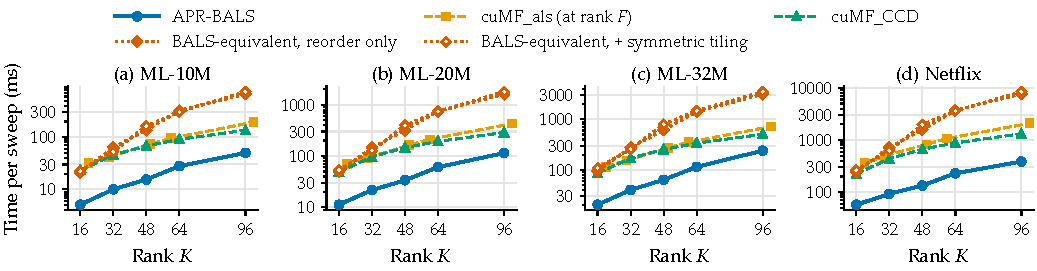
\includegraphics[width=\textwidth]{figures/fig_external.pdf}
\caption{Time per sweep of APR-BALS and three independent GPU systems on the RTX~3060 (log scale). cuMF\_als is plotted at its own rank $F \in \{20, 30, 50, 60, 100\}$, and cuMF\_CCD shows compute time per outer iteration. APR-BALS and cuMF\_als run without momentum. The cuMF\_CCD ratios in the text use the APR-BALS run with momentum, which is 0.4--2.9\% slower per sweep than the curve shown, so they are slightly more conservative than the figure. The BALS-equivalent kernels are our scalar FP32 reimplementation of BALS (Section~\ref{ssec:balsequiv}).}
\label{fig:external}
\end{figure*}

\subsection{Comparison with cuMF\_als}
\label{ssec:cumfals}

cuMF\_als \cite{tan2016faster} is the most widely cited GPU implementation of explicit-feedback ALS and uses the same weighted regularizer, run here with the same $\lambda = 0.048$. It supports ranks $F \in \{20, 30, 50, 60, 100\}$, paired here with $K \in \{16, 32, 48, 64, 96\}$, and solves each system with conjugate gradients. By \eqref{eq:gram_flops}, cuMF performs $1.51$, $0.88$, $1.08$, $0.88$, and $1.08$ times the Gram work of APR-BALS per rating at the five pairs, so cuMF does more Gram work at three pairs (up to $1.51\times$ at $K=16$) and 12\% less at two.

APR-BALS is faster per sweep at all 20 rank pairs, by $3.0\times$ to $6.4\times$ (Fig.~\ref{fig:external}). The margin is widest at $K=16$ ($5.6$--$6.4\times$), where cuMF also does the most extra Gram work. It is narrowest on ML-32M at $K \ge 64$ ($3.0$--$3.1\times$). Training RMSE differs by at most $0.52\%$ at $K \ge 32$, in the direction set by the rank mismatch; at $K=16$, cuMF's 25\% larger rank gives it a $1.4$--$2.2\%$ lower training error.

\textbf{Time to a common target.} Because conjugate gradients may do less work per sweep than an exact Cholesky solve, we also measured the time for each system to reach a common Netflix test RMSE, the worse of the two final values at each rank pair. At $K = 32$, 48, 64, and 96 the advantage equals or exceeds the per-sweep ratio: $7.17\times$, $6.15\times$, $6.19\times$, and $5.42\times$, against $5.38\times$, $6.15\times$, $4.64\times$, and $5.42\times$ per sweep. At $K{=}16$ it falls to $3.16\times$ (versus $6.33\times$), because cuMF's rank-20 model meets the target after 10 sweeps.

\textbf{Held-out accuracy.} On Netflix the two systems agree closely ($0.817559$ for APR-BALS at $K=96$ versus $0.817483$ for cuMF at $F=100$). On the MovieLens datasets cuMF reports a non-finite test RMSE, caused by items without a training rating (cold items), which our split allows. Under the weighted regularizer their systems are identically zero, so cuMF's conjugate-gradient step divides zero by zero, and its RMSE kernel's NaN guard is disabled by default; APR-BALS gives such items the uniform term, hence a zero factor. A direct count finds 30, 909, and 4{,}182 such items in ML-10M, ML-20M, and ML-32M, and none in Netflix, the one dataset on which cuMF's value is finite. Predicting zero for these ratings adds $0.02\%$, $0.20\%$, and $0.59\%$ to the APR-BALS test RMSE on the three MovieLens sets. The held-out comparison with cuMF therefore rests on Netflix, and the training-error comparison on all four large datasets.

\subsection{Comparison with cuMF\_CCD and cuMF\_SGD}
\label{ssec:ccdsgd}

The cuMF project also provides cuMF\_CCD, a GPU port of CCD++ \cite{yu2012scalable,nisa2017parallel}, and cuMF\_SGD \cite{xie2017cumf}. We converted each frozen split to their input formats and modified them only to build for sm\_86. cuMF\_CCD runs the same $K$ sweep for 15 outer iterations with its own $\lambda$ (0.05; 0.058 on Netflix). APR-BALS runs the shipped recipe (15 sweeps).

Averaged over the five ranks, APR-BALS is $3.83\times$, $3.72\times$, $3.44\times$, and $4.08\times$ faster than cuMF\_CCD on ML-10M, ML-20M, ML-32M, and Netflix. It is also more accurate at every matched $K$, although cuMF\_CCD uses its own $\lambda$ (Section~\ref{ssec:threats}). On Netflix, which has no cold items, the gap is clear ($0.8171$ versus $0.8267$ at $K=96$); on ML-32M it is about the size of the cold-item effect. The margin narrows with rank, from $3.9$--$4.5\times$ at $K=16$ to $2.1$--$3.3\times$ at $K=96$. This is consistent with the cost of a CCD++ sweep growing linearly in $K$ per rating, against quadratically for the Gram stage. BALS reported $2.09\times$, $3.86\times$, and $3.22\times$ over the same system on a TITAN~RTX for ML-10M, ML-20M, and Netflix \cite{chen2021bals}; the platforms differ, so this is not head-to-head.

cuMF\_SGD supports only $k=128$ and so has no curve in Fig.~\ref{fig:external}. Compared with APR-BALS at $K=96$, after 40 epochs it stays above the APR-BALS test RMSE on Netflix ($0.8221$ versus $0.8171$), although it spends less time. On ML-20M and ML-32M it trails by $0.25\%$ and $0.44\%$, comparable to the cold-item effect, and on ML-10M it is $0.08\%$ better and 11\% faster; we claim no accuracy advantage on MovieLens.

\subsection{Tensor Cores Versus the BALS Storage Format}
\label{ssec:balsequiv}

APR-BALS borrows its scalar storage format from BALS, so part of its advantage could come from the format rather than from the tensor cores. To separate the two, we built a faithful scalar-FP32 reimplementation of BALS in a separate binary. It uses the same tiled storage and shared-memory reuse, the frequency reordering of BALS, and, optionally, BALS's symmetric register-tile mapping, with no tensor cores. The BALS runs use an earlier initialization and different sweep counts, so we compare time per sweep.

The two BALS curves in Fig.~\ref{fig:external} yield two findings. First, symmetric tiling does not generalize on Ampere. It speeds up the reorder-only kernel by $1.08$--$1.21\times$ at $K=32$, but it is a net loss at 13 of the 20 dataset--rank pairs (down to $0.77\times$ at $K=48$), with identical sweep counts in both variants. Two opposing costs explain the pattern: idle threads in the triangular mapping ($3.20\times$ the live tiles at $K=16$) and, at $K \ge 48$, a lower occupancy ceiling ($66.7\%$ down to $41.7\%$); only at $K=32$ are both small. This finding concerns BALS's register mapping only, not its storage format or reordering, which both variants retain.

Second, the tensor-core dispatch accounts for most of the advantage over the BALS format, and its share grows with rank. Per sweep, APR-BALS is $4.1$--$4.7\times$ faster than the best BALS variant at $K=16$, $8.8$--$11.8\times$ at $K=48$, and $13.1$--$19.9\times$ at $K=96$; to convergence, the range is $3.5$--$29.9\times$. Because the storage format and reordering are common to both, the per-sweep ratio measures what the WMMA dispatch adds on top of BALS. It includes the host-level overhead removal of Section~\ref{ssec:nonsolver}, whose one separable part, the fast RMSE check, contributes $1.00\times$ at $K=16$ rising to about $1.10\times$ at $K \ge 48$. The rising ratio agrees with the kernel factor of Table~\ref{tab:precisioniso}. Finally, cuMF\_als is faster per sweep than the best BALS variant at $K \ge 32$ ($1.26$--$1.67\times$ at $K=32$); the original BALS evaluation did not include cuMF\_als.

\subsection{Threats to Validity}
\label{ssec:threats}

\textbf{Hardware scope.} We tested only an RTX~3060 (Ampere) and a Tesla~T4 (Turing), not data-center parts such as the A100 or H100, whose FP16-to-FP32 throughput ratios and memory bandwidths differ substantially, or non-NVIDIA matrix engines.

\textbf{Problem scope.} Only $K \in \{16, 32, 48, 64, 96\}$ is supported. The restriction follows from the $16 \times 16 \times 16$ WMMA shape; other multiples of 16 need only a new template instantiation and a spill check, and other ranks would need zero padding, which is not implemented. We handle explicit feedback on a single GPU. Implicit-feedback objectives change the Gram structure the dispatch relies on, and multi-GPU partitioning is untested.

\textbf{Measurement limits.} Atomic additions in the scalar kernel make both paths reproducible only to about $10^{-6}$ in RMSE, and no claim finer than that is made. Only the two-path wall times (Table~\ref{tab:main3060}) are five-run measurements; the other timings are single runs, the hardware counters are single launches, and the $\lambda$ sweep covers only $K=96$ on two datasets. Finally, the three isolation measures answer different questions: at Netflix $K=96$ the two-path harness gives $14.8\times$ end to end, the kernel ablation $17.8\times$ on the Gram-and-solve phase, and the BALS comparison $19.9\times$ per sweep. None substitutes for another.

\textbf{Baseline and protocol.} The FP32 baseline is slower than cuMF\_als at $K \ge 32$ (Section~\ref{ssec:scalar}), and the kernel factor of Table~\ref{tab:precisioniso} bundles the tensor pipe with the WMMA dataflow. $\lambda$ was selected on the test ratings, which may favour APR-BALS in the accuracy comparisons with cuMF\_CCD and cuMF\_SGD. Convergence is checked every five sweeps, so sweep counts are quantized; the momentum gain and the fixed-iteration cuMF\_CCD comparison depend on it.
